\section[Tipos de Intercambio de Energía entre Sistemas Termodinámicos]
 {Tipos de Intercambio de Energía\\entre Sistemas Termodinámicos}

\begin{enumerate}
	\item El intercambio de energía de tipo calor, tiene más de una modalidad.\\
	      Una de estas es llamada ``conducción''. Por ejemplo, considerando la
	      siguiente situación:

	      \begin{center}
		      \begin{tikzpicture}
			      \draw (0,0) -- (0,2) -- (2,2) -- (2,0) -- (0,0);
			      \draw (-1,1) node {$T_A$};
			      \draw (3,1) node {$T_B$};
			      \draw (0.5,1.6) node {$A$};
			      \draw (1.5,1.6) node {$B$};

			      \draw (0.9,0) -- (0.9,2);
			      \draw (1.1,0) -- (1.1,2);

			      \draw[ ->, azulito ] (1,1.5) to[bend right] (1.6,2.2)
			      node [above] {$A_C$};

			      \draw[|-|] (0.9,-0.2) -- (1.1,-0.2) node[midway, yshift=-8] {$\Delta x$};
			      \draw[ ->, amarillito ] (0.55,1) -- (1.05,1.1) -- (0.95,0.9) -- (1.55,1);
			      \node at (0.4,0.7) {$\Delta Q$};
		      \end{tikzpicture}
	      \end{center}

	      Un bloque de un mismo material, una de sus caras se encuentra a una
	      temperatura $T_A$ y la opuesta a una temperatura $T_B$, y centrandonos
	      en un pedazo del bloque con ancho $\Delta x$ y área $A_C$. Como las
	      temperaturas son diferentes, hay un flujo de calor. En este caso
	      (conducción), se cumple que:
	      \[\odv{Q}{t} = k\,A_C\,\odv{T}{x}\]
	      Donde $k$ resulta ser la conductividad térmica de la sustancia del bloque.
	      Nótese que $[k] = \si{\watt\per{\m\kelvin}}$.

	      \subsection{Ejemplo Numéríco: Conductividad}

Una ventana de espesor $L=\qty{2}{\mm}$, con sección transversal
$A_C = \qty{2e6}{\mm^2}$, conductividad térmica
$k = \qty{0.8}{\watt\per{\m\kelvin}}$. Sometida a una temperatura
constante por un lado $T_A = \qty{20}{\degreeCelsius}$ y por el otro a
una temperatura $T_B=\qty{15}{\degreeCelsius}$. Hallar $T$ en
$x=\qty{1}{\mm}$. Bajo estas condiciones, se tiene que el término
$\ds\odv{T}{x}$ es constante, pues de no ser así, se podría pensar en cada
sección de la ventana como un subsistema, el cual estaría cambiando de
temperatura, lo que, por segunda ley de la termidinámica, entraría en
contradicción con la suposición de que $T_A$ y $T_B$ permanecen
constantes.

Así, se tiene entonces que la temperatura en función de la distancia se
comporta de manera lineal. Como se conocen las temperaturas de los
extemos en contacto con ambas temperaturas, se pueden usar para
determinar este comportamiento:
\[
    \begin{derivation}
            \res{ \odv{T}{x} = \alpha }\\
        \equiv\\
            \res{ \odv{T}{x} = \frac{\Delta T}{\Delta x} }\\
        \To\\
            \res{ \odv{T}{x} = \frac{T_A - T_B}{-L} }\\
        \equiv\\
            \res{ \odv{T}{x} = -\qty{2.5}{\degreeCelsius\per\mm} }
    \end{derivation}
\]

Por la misma razón, se debe mantener la igualdad cuando se toma, en vez
de $(L,T_B)$ para hallar la razón, $(x,T(x))$, en especial, para el $x$
de interés:
\[
    \begin{derivation}
            \res{ -\qty{2.5}{\degreeCelsius\per\mm} 
            = \frac{\qty{20}{\degreeCelsius} - T(\qty{2}{\mm})}{-\qty{2}{\mm}} }\\
        \equiv\\
            \res{ T(\qty{2}{\mm}) = \qty{15}{\degreeCelsius} }
    \end{derivation}
\]

Por otra parte, como se tienen los valores de $k$, $A_C$ y 
$\ds\odv{T}{x}$, entonces
\[
    \begin{derivation}
            \res{ \odv{Q}{t} = k\,A_C\,\odv{T}{x} }\\
        \equiv\\
            \res{ \odv{Q}{t} = -\qty{4e3}{\watt} }
    \end{derivation}
\]

Volviendo a un caso general, la ecuación bajo la condición de que las
temperaturas de los extremos permanece constante se puede escribir como
\[\odv{Q}{t} = A_C\,\frac{T_A - T_B}{L/k}\]
Donde $\dfrac{L}{k}$ se conoce como la resistencia térmica ($R$). Esta
resistencia, al depender de $k$ y $L$, caracterizan una lámina de un
material. En un sistema donde hay múltiples lámines en serie, la
resistencia térmica total es la suma de las resistencias de sus láminas.

	\item Otra forma de transferencia de calor es mediante procesos llamados
	      convectivos. Estos procesos no tienen una única descripción matemática,
	      sin embargo, siempre implican una transferencia de masa de uno de los
	      sistemas al otro:
	      \begin{center}
		      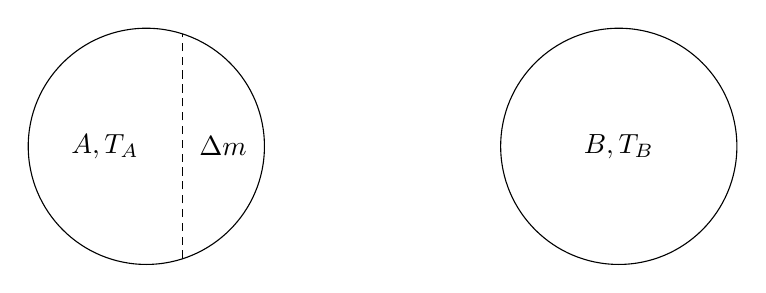
\begin{tikzpicture}[scale=1.5]
			      \draw (-2,0) circle (1);
			      \draw (2,0) circle (1)
			      node {$B,T_B$};

			      \node at (-2.35, 0) {$A,T_A$};
			      \node at (-1.35, 0) {$\Delta m$};

			      \draw[densely dashed] (-1.69098301,-0.951056516) -- (-1.69098301,0.951056516);
		      \end{tikzpicture}

		      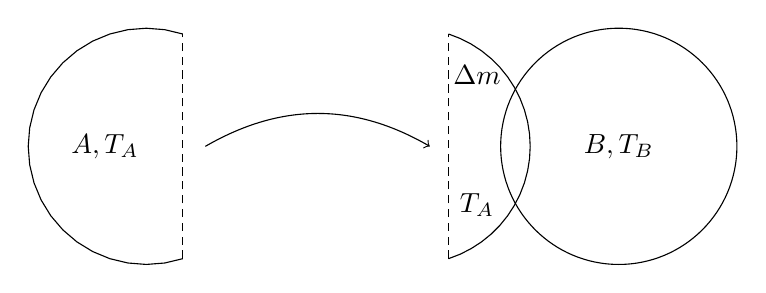
\begin{tikzpicture}[scale=1.5]
			      \draw[domain=72:288] plot ({cos(\x)-2},{sin(\x)});
			      \draw[domain=-72:72] plot ({cos(\x)+0.25},{sin(\x)});
			      \draw (2,0) circle (1)
			      node {$B,T_B$};

			      \node at (-2.35, 0) {$A,T_A$};
			      \node at (0.8, 0.6) {$\Delta m$};
			      \node at (0.8, -0.5) {$T_A$};

			      \draw[densely dashed] (-1.69098301,-0.951056516) -- (-1.69098301,0.951056516);
			      \draw[densely dashed] (0.559016994,-0.951056516) -- (0.559016994,0.951056516);

			      \draw[ -> ] (-1.5,0) to[bend left] (0.4,0);
		      \end{tikzpicture}
	      \end{center}
	      La complejidad de estos procesos está en que dependen de la geometría
	      de ambos sistemas, sus composiciónes y propiedades superficiales.
	      Algunas de las características comunes de estos procesos son las siguientes:
	      \begin{enumerate}
		      \item Al estar un fluido en contacto con una superficie, la tasa de
		            transferencia de calor es proporcional a la superfice de contacto.
		      \item la viscosidad de un fluido genera películas en la superficie,
		            lo que afecta a la transferencia de calor a este. La velocidad del
		            fluido tiende a disminuir esta película, mejorando la transferencia
		            de calor.
					\item \[\Exists{\upalpha}{\odv{Q}{t} \approx \upalpha(T_S - T_F)^{1.25}}\]
					Esta constante $\upalpha$ depende de cada caso.
	      \end{enumerate}
				\item Otra forma de transferencia se da por radiación electromagnética.
							La descripción matemática de esta viene dada por las siguientes
							constantes:

							\begin{tabular}{ |L|L|l| }
								\hline
								\text{variable}	& \text{valor}	& Nombre o Significado\\
								\hline
								\upsigma	& \qty{5.67e-8}{\watt\per{\m^2(\kelvin)^4}}	& Constante de Stefan - Boltzmann\\
								\upvarepsilon & 0 < \upvarepsilon \leq 1	& Emisividad\\
								A_S	& \rule[1pt]{40pt}{1pt}	& Área superficial del cuerpo\\
								T	&	\rule[1pt]{40pt}{1pt} & Temperatura absoluta del cuerpo\\
								\hline
							\end{tabular}

							Y su expresión es:
							\[\odv{Q}{t} = \upsigma\,\upvarepsilon\,A_S\,T^4\]
							Donde $Q$ se refiere al calor, sin embargo, es energía en general.
							\subsection{Ejemplo Numérico: Radiación}

Considerando una sartén de aluminio a \qty{373.15}{\kelvin} en un entorno a
temperatura ambiente de \qty{288.15}{\kelvin}. Si el área superficial
de la sartén es de \qty{100}{\cm^2}. La potencia que le entrega la
sartén al entorno es:
\[
  \begin{derivation}
      \res{ \odv{Q}{t} = \upsigma\,\upvarepsilon\,A_S\,(T_s^4 - T_a^4) }\\
    \equiv\\
      \res{ \odv{Q}{t} = (\num{5.67e-8})(0.03)(100)(373.15^4 - 288.15^4) }\\
    \equiv\\
      \res{ \odv{Q}{t} = \qty{2.125}{\watt} }
  \end{derivation}
\]
				\item Transferencia de energía por trabajo mecánico: 
							considerando un sistema $A$ rodeado por un entorno $E$,
							con energías $U_A$, $U_E$ respectivamente. El sistema $A$
							podría deformar al entorno, y esta deformación estaría
							caracterizada por una distancia $\Updelta x$ y un área
							transversal $\Updelta A_{s,t}$. Para poder lograr esta
							deformación, el sistema $A$ debe ejercer una fuerza $F$
							al entorno.

							De igual manera, puede ocurrir en el otro sentido, esto
							es, que el entorno deforme al sistema $A$.

							A esta fuerza se le puede asociar un trabajo $T_r$ y
							\[
								\begin{derivation}
										\res{ \Updelta T_r = F \Updelta x }\\
									\why[\To]{Sumando para toda la deformación y reduciendo $\Updelta x$}\\
										\res{ T_r = \int F \,\diff{x} }\\
									\equiv\\
										\res{ T_r = \int \frac{F}{\Updelta A_{s,t}}\Updelta A_{s,t}\,\diff{x}}\\
									\why{ $P = F/A$ , $V = L\,A$}\\
										\res{ T_r = \int p \,\diff{V} }
								\end{derivation}
							\]
							Por convención, la presión a la que se refiere es a la
							ejercida por el sistema al entorno, lo que resulta en
							que el valor de esta sea negativo, pues se está viendo
							desde el punto de vista del sistema.

							\[T_r = -\int p\,\diff{x}\]
\end{enumerate}

Considerando ahora solo transferencias de energía de tipo calor y
mecánicas, la primera ley de la termodinámica se puede reescribir como:

La energía $U$ del universo se conserva, y desde el punto de vista de un
sistema $A$, las absorsiones de este se tomarán positivas. Entonces,
si $A$ recibe un calor $Q$ y el entorno es el que ejerce un trabajo
sobre $A$, se considera positivo.

